\documentclass{vkr}
\usepackage[english, russian]{babel} % переносы
\usepackage{graphicx} % для вставки картинок
\graphicspath{{images/}} % путь к изображениям
\usepackage[hidelinks]{hyperref}
\usepackage{float} % определяет метод H для рисунка с переносом на следующую страницу, ели не помещается
\usepackage{pdflscape}
\addto{\captionsrussian}{\renewcommand{\refname}{СПИСОК ИСПОЛЬЗОВАННЫХ ИСТОЧНИКОВ}}
\usepackage{xltabular} % для вставки таблиц
\usepackage{makecell}
\renewcommand\theadfont{} % шрифт в /thead
\usepackage{array} % для определения новых типов столбцов таблиц
\newcolumntype{T}{>{\centering\arraybackslash}X} % новый тип столбца T - автоматическая ширина столбца с выравниванием по центру
\newcolumntype{R}{>{\raggedleft\arraybackslash}X} % новый тип столбца R - автоматическая ширина столбца с выравниванием по правому краю
\newcolumntype{C}[1]{>{\centering\let\newline\\\arraybackslash\hspace{0pt}}m{#1}} % новый тип столбца C - фиксированная ширина столбца с выравниванием по центру
\newcolumntype{r}[1]{>{\raggedleft\arraybackslash}p{#1}} % новый тип столбца r - фиксированная ширина столбца с выравниванием по правому краю
\newcommand{\centrow}{\centering\arraybackslash} % командой \centrow можно центрировать одну ячейку (заголовок) в столбце типа X или p, оставив в оcтальных ячейках другой тип выравнивания
\newcommand{\finishhead}{\endhead\hline\endlastfoot}
\newcommand{\continuecaption}[1]{\caption*{#1}\\ \hline }
\usepackage{etoolbox}
\AtBeginEnvironment{xltabular}{\refstepcounter{tablecnt}} % подсчет таблиц xltabular, обычные таблицы подсчитываются в классе

\usepackage[tableposition=top]{caption} % подпись таблицы вверху
\captionsetup{strut=off}
\setlength{\intextsep}{0pt} % Vertical space above & below [h] floats
\setlength{\textfloatsep}{0pt} % Vertical space below (above) [t] ([b]) floats
\DeclareCaptionLabelFormat{gostfigure}{Рисунок #2} %подпись рисунка
\DeclareCaptionLabelFormat{gosttable}{Таблица #2} %подпись таблицы
\DeclareCaptionLabelSeparator{gost}{~--~} %разделитель в рисунках и таблицах
\captionsetup{labelsep=gost}
\captionsetup[figure]{aboveskip=10pt,belowskip=4mm,justification=centering,labelformat=gostfigure} % настройка подписи рисунка
\captionsetup[table]{font={stretch=1.41},skip=0pt,belowskip=0pt,aboveskip=8.5pt,singlelinecheck=off,labelformat=gosttable} % настройка подписи таблицы

\setlength{\LTpre}{8mm} % отступ сверху таблицы
\setlength{\LTpost}{6mm} % отступ снизу таблицы

\usepackage{enumitem}
\setlist{nolistsep,wide=\parindent,itemindent=*} % отступы вокруг списков, выравнивание с учетом разделителя

\usepackage{color} %% это для отображения цвета в коде
\usepackage{listings} %% листинги кода
\setmonofont[Scale=0.7]{Verdana} % моноширный шрифт для листинга

\definecolor{codegreen}{rgb}{0,0.6,0}
\definecolor{codegray}{rgb}{0.5,0.5,0.5}
\definecolor{codepurple}{rgb}{0.58,0,0.82}

\lstset{ %
language=C,                 % выбор языка для подсветки (здесь это С)
numbers=left,               % где поставить нумерацию строк (слева\справа)
numberstyle=\tiny,           % размер шрифта для номеров строк
stepnumber=1,                   % размер шага между двумя номерами строк
numbersep=5pt,                % как далеко отстоят номера строк от подсвечиваемого кода
commentstyle=\color{codegreen},
keywordstyle=\color{magenta},
numberstyle=\tiny\color{codegray},
stringstyle=\color{codepurple},
basicstyle=\linespread{0.95}\ttfamily,
backgroundcolor=\color{white}, % цвет фона подсветки - используем \usepackage{color}
showspaces=false,            % показывать или нет пробелы специальными отступами
showstringspaces=false,      % показывать или нет пробелы в строках
showtabs=false,             % показывать или нет табуляцию в строках
frame=single,              % рисовать рамку вокруг кода
tabsize=2,                 % размер табуляции по умолчанию равен 2 пробелам
captionpos=t,              % позиция заголовка вверху [t] или внизу [b] 
breaklines=true,           % автоматически переносить строки (да\нет)
breakatwhitespace=false, % переносить строки только если есть пробел
escapeinside={\%*}{*)}   % если нужно добавить комментарии в коде
}

\makeatletter % чтобы допускались русские комментарии в листингах
\lst@InputCatcodes
\def\lst@DefEC{%
 \lst@CCECUse \lst@ProcessLetter
  ^^80^^81^^82^^83^^84^^85^^86^^87^^88^^89^^8a^^8b^^8c^^8d^^8e^^8f%
  ^^90^^91^^92^^93^^94^^95^^96^^97^^98^^99^^9a^^9b^^9c^^9d^^9e^^9f%
  ^^a0^^a1^^a2^^a3^^a4^^a5^^a6^^a7^^a8^^a9^^aa^^ab^^ac^^ad^^ae^^af%
  ^^b0^^b1^^b2^^b3^^b4^^b5^^b6^^b7^^b8^^b9^^ba^^bb^^bc^^bd^^be^^bf%
  ^^c0^^c1^^c2^^c3^^c4^^c5^^c6^^c7^^c8^^c9^^ca^^cb^^cc^^cd^^ce^^cf%
  ^^d0^^d1^^d2^^d3^^d4^^d5^^d6^^d7^^d8^^d9^^da^^db^^dc^^dd^^de^^df%
  ^^e0^^e1^^e2^^e3^^e4^^e5^^e6^^e7^^e8^^e9^^ea^^eb^^ec^^ed^^ee^^ef%
  ^^f0^^f1^^f2^^f3^^f4^^f5^^f6^^f7^^f8^^f9^^fa^^fb^^fc^^fd^^fe^^ff%
  ^^^^20ac^^^^0153^^^^0152%
  % Basic Cyrillic alphabet coverage
  ^^^^0410^^^^0411^^^^0412^^^^0413^^^^0414^^^^0415^^^^0416^^^^0417%
  ^^^^0418^^^^0419^^^^041a^^^^041b^^^^041c^^^^041d^^^^041e^^^^041f%
  ^^^^0420^^^^0421^^^^0422^^^^0423^^^^0424^^^^0425^^^^0426^^^^0427%
  ^^^^0428^^^^0429^^^^042a^^^^042b^^^^042c^^^^042d^^^^042e^^^^042f%
  ^^^^0430^^^^0431^^^^0432^^^^0433^^^^0434^^^^0435^^^^0436^^^^0437%
  ^^^^0438^^^^0439^^^^043a^^^^043b^^^^043c^^^^043d^^^^043e^^^^043f%
  ^^^^0440^^^^0441^^^^0442^^^^0443^^^^0444^^^^0445^^^^0446^^^^0447%
  ^^^^0448^^^^0449^^^^044a^^^^044b^^^^044c^^^^044d^^^^044e^^^^044f%
  ^^^^0401^^^^0451%
  %%%
  ^^00}
\lst@RestoreCatcodes
\makeatother


% Режим шаблона (должен быть включен один из трех)
%\ВКРtrue
%\Практикаtrue
\Курсоваяtrue

\newcommand{\Дисциплина}{<<Проектирование и архитектура программных систем>>} % для курсовой
\newcommand{\КодСпециальности}{09.03.04} % Курсовая
\newcommand{\Специальность}{Программная инженерия} % Курсовая
\newcommand{\Тема}{Веб мессенджер} % ВКР Курсовая
\newcommand{\ГдеПроводитсяПрактика}{Юго-Западном государственном университете} % для практики
\newcommand{\РуководительПрактПредпр}{Куркина А. В.} % для практики
\newcommand{\ДолжнРуководительПрактПредпр}{директор} % для практики
\newcommand{\РуководительПрактУнивер}{Чаплыгин А. А.} % для практики
\newcommand{\ДолжнРуководительПрактУнивер}{к.т.н. доцент} % для практики
\newcommand{\Автор}{Б.Р. Якубов}
\newcommand{\АвторРод}{Якубова Б.Р.}
\newcommand{\АвторПолностьюРод}{Иванова Ивана Ивановича} % для практики
\newcommand{\Шифр}{21-06-0052}
\newcommand{\Курс}{3} % для практики
\newcommand{\Группа}{ПО-12б}
\newcommand{\Руководитель}{А. А. Чаплыгин} % для ВКР и курсовой
\newcommand{\Нормоконтроль}{А. А. Чаплыгин} % для ВКР
\newcommand{\ЗавКаф}{А. В. Малышев} % для ВКР
\newcommand{\ДатаПриказа}{«07» апреля 2023~г.} % для ВКР
\newcommand{\НомерПриказа}{1505-с} % для ВКР
\newcommand{\СрокПредоставления}{«11» января 2024~г.} % для ВКР, курсового

\begin{document}
\maketitle
\ifПрактика{}\else{
   \newpage
\begin{center}
	\large\textbf{Минобрнауки России}
	
	\large\textbf{Юго-Западный государственный университет}
	\vskip 1em
	\normalsize{Кафедра программной инженерии}
	\vskip 1em
	\ifВКР{
		\begin{flushright}
			\begin{tabular}{p{.4\textwidth}}
				\centrow УТВЕРЖДАЮ: \\
				\centrow Заведующий кафедрой \\
				\hrulefill \\
				\setarstrut{\footnotesize}
				\centrow\footnotesize{(подпись, инициалы, фамилия)}\\
				\restorearstrut
				«\underline{\hspace{1cm}}»
				\underline{\hspace{3cm}}
				20\underline{\hspace{1cm}} г.\\
			\end{tabular}
		\end{flushright}
	}\fi
\end{center}
\vspace{1em}
\begin{center}
	\large
	\ifВКР{
		ЗАДАНИЕ НА ВЫПУСКНУЮ КВАЛИФИКАЦИОННУЮ РАБОТУ
		ПО ПРОГРАММЕ БАКАЛАВРИАТА}
	\else
	ЗАДАНИЕ НА КУРСОВУЮ РАБОТУ (ПРОЕКТ)
	\fi
	\normalsize
\end{center}
\vspace{1em}
{\parindent0pt
	Студента \АвторРод, шифр\ \Шифр, группа \Группа
	
	1. Тема «\Тема\ \ТемаВтораяСтрока»
	\ifВКР{
		утверждена приказом ректора ЮЗГУ от \ДатаПриказа\ № \НомерПриказа
	}\fi.
	
	2. Срок предоставления работы к защите \СрокПредоставления
	
	3. Исходные данные для создания программной системы:
	
	3.1. Перечень решаемых задач:}

\renewcommand\labelenumi{\theenumi)}

\begin{enumerate}
	\item ознакомиться с обработкой веб запросов;
	\item разработать серверную часть приложения;
	\item разработать клиентскую часть приложения;
	\item Доработать мессенджер и провести тестирование.
\end{enumerate}

{\parindent0pt
	3.2. Входные данные и требуемые результаты для программы:}

\begin{enumerate}
	\item Входными данными у мессенджера является возможность писать а так же принимать сообщения так же необходима система регистрации и входа, дабы отличать пользователей по их именам или же никнеймам. 
%	Выходными данными являются графическая интерпретация игрового процесса на мониторе пользователя. Действия игрока влияют на игровой про-цесс и текущее состояние игровой сцены. Игрок контролирует автомобиль с помощью интерфейса пользователя.
	
	\item  выходными данными являтеся тот факт что пользователь взаимодействует с приложением, предоставляя данные для регистрации, входа и отправки сообщений, и ожидает соответствующих результатов в виде успешных операций.
\end{enumerate}

{\parindent0pt
	
	4. Содержание работы (по разделам):
	
	4.1. Введение
	
	4.2. Анализ предметной области
	
	4.3. Техническое задание: основание для разработки, назначение разработки,
	требования к программной системе, требования к оформлению документации.
	
	4.4. Технический проект: общие сведения о программной системе, проект
	данных программной системы, проектирование архитектуры программной системы, проектирование пользовательского интерфейса программной системы.
	
	4.5. Рабочий проект: спецификация компонентов и классов программной системы, тестирование программной системы, сборка компонентов программной системы.
	
	4.6. Заключение
	
	4.7. Список использованных источников
	

	
	\списокПлакатов
	
	\vskip 2em
	\begin{tabular}{p{6.8cm}C{3.8cm}C{4.8cm}}
		Руководитель \ifВКР{ВКР}\else работы (проекта) \fi & \lhrulefill{\fill} & \fillcenter\Руководитель\\
		\setarstrut{\footnotesize}
		& \footnotesize{(подпись, дата)} & \footnotesize{(инициалы, фамилия)}\\
		\restorearstrut
		Задание принял к исполнению & \lhrulefill{\fill} & \fillcenter\Автор\\
		\setarstrut{\footnotesize}
		& \footnotesize{(подпись, дата)} & \footnotesize{(инициалы, фамилия)}\\
		\restorearstrut
	\end{tabular}
}

\renewcommand\labelenumi{\theenumi.}

   \abstract{РЕФЕРАТ}

Объем работы равен \formbytotal{lastpage}{страниц}{е}{ам}{ам}. Работа содержит \formbytotal{figurecnt}{иллюстраци}{ю}{и}{й}, \formbytotal{tablecnt}{таблиц}{у}{ы}{}, \arabic{bibcount} библиографических источников. Количество приложений – 1. Фрагменты исходного кода представлены в приложении А. 

Перечень ключевых слов: Веб-приложение, мессенджер, JavaScript, HTML, CSS, frontend, регистрация пользователя, вход в систему, чат, отправка сообщений, AJAX, Fetch API, асинхронное программирование, WebSockets, серверная часть, Python, SQLite, Waitress, web-разработка, RESTful API, аутентификация, безопасность, клиент-серверное взаимодействие, URL-маршрутизация, реальное время.

Объектом разработки является веб-приложение мессенджера, предоставляющее современные возможности обмена сообщениями и взаимодействия пользователей в режиме реального времени.

Целью проекта является создание удобного и функционального мессенджера, способного обеспечить эффективное общение пользователей, а также привлечь новых пользователей своей удобной и привлекательной функциональностью.

В процессе разработки был создан веб-приложение а так же сервер с использованием современных технологий, таких как JavaScript, HTML, CSS и Python. Реализованы основные элементы мессенджера, включая чат, отправку сообщений, систему регистрации и входа в систему.

При разработке использовались технологии веб-разработки, обеспечивающие асинхронное взаимодействие и удобный пользовательский интерфейс.

Разработанное веб-приложение успешно прошло этапы тестирования и полностью готова к полноценной эксплуатации.

\selectlanguage{english}
\abstract{ABSTRACT}

The volume of work is \formbytotal{lastpage}{page}{}{s}{s}. The work contains \formbytotal{figurecnt}{illustration}{}{s}{s}, \formbytotal{tablecnt}{table}{}{s}{s}, \arabic{bibcount} bibliographic sources. The number of applications is 1. The layout of the site, including the connection of components, is presented in annex A.

List of keywords: Web application, messenger, JavaScript, HTML, CSS, frontend, user registration, login, chat, sending messages, AJAX, Fetch API, asynchronous programming, WebSockets, server side, Python, SQLite, Waitress, web development, RESTful API, authentication, security, client-server interaction, URL routing, real time.

The object of development is a web-based messenger application that provides modern messaging and user interaction in real time.

The goal of the project is to create a convenient and functional messenger capable of providing effective user communication, as well as attracting new users with its convenient and attractive functionality.

In the process of development was created a web application and a server using modern technologies such as JavaScript, HTML, CSS and Python. The main elements of the messenger were realized, including chat, sending messages, registration and login system.

Web development technologies were used during the development, providing asynchronous interaction and a convenient user interface.

The developed web application has successfully passed the testing stages and is fully ready for full-scale operation.

\selectlanguage{russian}
}\fi
\tableofcontents
\section*{ОБОЗНАЧЕНИЯ И СОКРАЩЕНИЯ}

ПО -- программное обеспечение.

РП -- рабочий проект.

ТЗ -- техническое задание.

ТП -- технический проект.

UML (Unified Modelling Language) -- язык графического описания для объектного моделирования в области разработки программного обеспечения.

\ifПрактика{}\else{\section*{ВВЕДЕНИЕ}
\addcontentsline{toc}{section}{ВВЕДЕНИЕ}


В современном мире информационных технологий веб-мессенджеры стали неотъемлемой частью нашей повседневной жизни. За последние десятилетия создание мессенджеров стало одним из самых востребованных направлений в программировании. Искусство разработки мессенджеров предоставляет уникальную возможность соединить техническое мастерство с креативностью и фантазией. В рамках данного курсового проекта мы погрузимся в увлекательный мир разработки веб-мессенджера и рассмотрим процесс создания современного приложения для обмена сообщениями с использованием технологий веб-разработки.

Наш веб-мессенджер предназначен для обеспечения эффективного и удобного общения пользователей в режиме реального времени, а также привлечения новых пользователей своей функциональностью и привлекательным дизайном.

В процессе разработки было создано веб-приложение, использующее современные веб-технологии, включая JavaScript, HTML и CSS. Реализованы основные элементы мессенджера, такие как чат, отправка сообщений, система регистрации и входа в систему.

При разработке использовались современные технологии веб-разработки, а также библиотеки и фреймворки, обеспечивающие удобный пользовательский интерфейс и безопасное взаимодействие.


\emph{Цель настоящей работы} –  создание современного веб-мессенджера с использованием технологий веб-разработки. Для достижения этой цели необходимо решить \emph{следующие задачи:}
\begin{itemize}
	\item провести анализ современных веб-мессенджеров;
	\item разработать концепцию и функциональные требования к мессенджеру;
	\item спроектировать веб-приложение с учетом требований безопасности и удобства использования;
	\item реализовать функционал мессенджера.
\end{itemize}

\emph{Структура и объем проекта.} Проект включает в себя введение, 4 раздела основной части, заключение, список использованных технологий, 2 приложения. Общий объем проекта равен \formbytotal{page}{страниц}{е}{ам}{ам}.

\emph{Во введении} сформулирована цель проекта, поставлены задачи разработки, описана структура проекта, приведено краткое содержание каждого из разделов.

\emph{В первом разделе} производится анализ существующих веб-мессенджеров и их технических характеристик.

\emph{Во втором разделе} формулируются требования к создаваемому веб-мессенджеру на этапе технического задания.

\emph{В третьем разделе} представлен детальный технический проект, включая выбор используемых технологий, архитектуру приложения и основные функциональные блоки.

\emph{В четвертом разделе} представлен исходный код разработанного мессенджера, проведено тестирование и оценка его производительности.

В заключении изложены основные результаты проекта, полученные в ходе разработки.

В приложении А представлен исходный код.
 
}\fi
\section{Анализ предметной области}
\subsection{История развития веб-мессенджеров}

История веб-мессенджеров тесно связана с развитием интернет-технологий и появлением средств онлайн-коммуникации. Этот жанр программного обеспечения стал неотъемлемой частью современного общения в виртуальном пространстве. Вот краткая история развития веб-мессенджеров:

\begin{enumerate}
	\item \textbf{IRC и ICQ (1990-е годы):} Первыми формами онлайн-чата были интернет-ретрансляции (IRC), позволяющие пользователям общаться в реальном времени. В середине 1990-х годов появилась ICQ, первая широко распространенная программа мгновенного обмена сообщениями, что сделало общение в сети более доступным.
	
	\item \textbf{AIM, MSN Messenger, Yahoo Messenger (2000-е годы):} В 2000-х годах появились AIM (AOL Instant Messenger), MSN Messenger и Yahoo Messenger. Они предложили дополнительные функции, такие как передача файлов, видеозвонки и персонализированные статусы.
	
	\item \textbf{Skype и Google Talk (2000-е годы):} Skype и Google Talk (позднее ставший частью Google Hangouts) предоставили пользователям возможность совершения голосовых и видеозвонков, расширяя возможности коммуникации.
	
	\item \textbf{WhatsApp, Telegram, и Viber (2010-е годы):} С массовым распространением смартфонов в 2010-х годах, приложения мессенджеров на основе мобильных платформ, такие как WhatsApp, Telegram и Viber, стали популярными, предлагая шифрование сообщений и другие расширенные функции.
	
	\item \textbf{Современные веб-мессенджеры (2020-е годы):} С появлением современных веб-мессенджеров, таких как Slack, Microsoft Teams, и Discord, область коммуникаций в корпоративном и геймерском сегментах значительно разнообразилась. Эти приложения интегрируют функциональности чата с коллективной работой, обменом файлами и другими возможностями.
	
\end{enumerate}

История веб-мессенджеров демонстрирует постоянное развитие средств онлайн-коммуникации, от простых текстовых чатов до многофункциональных приложений, объединяющих в себе различные аспекты виртуального общения.

\subsection{Веб-мессенджер: особенности и тенденции}
Веб-мессенджер – это приложение, предназначенное для обмена мгновенными сообщениями в режиме реального времени через сеть интернет. Основные особенности и тенденции веб-мессенджеров включают:

\begin{enumerate}
	\item \textbf{Многоплатформенность:} Современные веб-мессенджеры обеспечивают поддержку различных платформ, включая веб-версии, мобильные приложения и настольные приложения.
	
	\item \textbf{Безопасность и шифрование:} В ответ на повышенный интерес к безопасности в сети, веб-мессенджеры внедряют технологии шифрования сообщений для защиты конфиденциальности пользователей.
	
	\item \textbf{Интеграция с другими сервисами:} Современные мессенджеры предоставляют интеграцию с другими сервисами и приложениями, такими как облачные хранилища, календари, видеоконференции, что обогащает опыт пользователей.
	
	\item \textbf{Коллективная работа:} Веб-мессенджеры для бизнеса (например, Slack, Microsoft Teams) акцентируют внимание на коллективной работе, предоставляя инструменты для обмена файлами, обсуждения проектов и интеграции с рабочими инструментами.
	
	\item \textbf{Использование искусственного интеллекта:} Некоторые веб-мессенджеры начинают использовать искусственный интеллект для улучшения опыта пользователей, предоставляя персонализированные рекомендации и автоматизированные задачи.
	
\end{enumerate}

Тенденции веб-мессенджеров продолжают эволюцию в ответ на изменяющиеся потребности пользователей и бизнеса, что подчеркивает их важность в современной коммуникационной экосистеме.

\begin{figure}
	\centering
	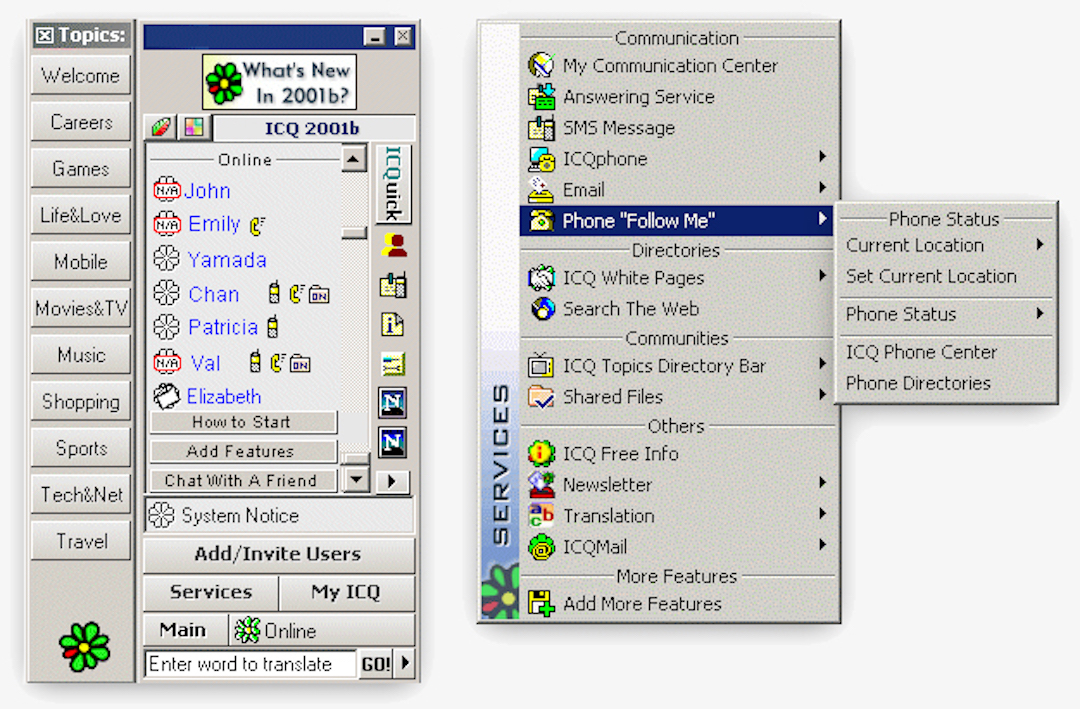
\includegraphics[width=0.7\linewidth]{images/icq}
	\caption{Первый мессенджер ICQ}
	\label{fig:icq}
\end{figure}

\begin{figure}
	\centering
	
\includegraphics[width=0.7\linewidth]{images/telegram}
	\caption{Популярный мессенджер Telegram}
	\label{fig:telegram}
\end{figure}

\section{Техническое задание}
\subsection{Основание для разработки}

Основанием для разработки является потребность в создании веб-мессенджера в рамках проекта по предмету "Проектирование и разработка программных систем".

\subsection{Цель и назначение разработки}

Основной целью данного проекта является разработка веб-мессенджера с использованием технологий Python для серверной части, а также JavaScript, HTML и CSS для клиентской части.

Целью разработки веб-мессенджера является предоставление эффективного инструмента для обмена мгновенными сообщениями в веб-пространстве, обеспечивая удобство использования и современные функциональные возможности.

Задачи данной разработки включают:
\begin{itemize}
	\item Создание серверной части мессенджера на языке Python, обеспечивающей обработку сообщений, управление пользователями и хранение данных.
	\item Разработка клиентской части веб-мессенджера, используя JavaScript, HTML и CSS для обеспечения удобного пользовательского интерфейса.
	\item Реализация механизмов обмена сообщениями в режиме реального времени.
	\item Обеспечение безопасности обмена данными и внедрение технологий шифрования для защиты конфиденциальности.
	\item Тестирование и отладка системы для выявления и устранения возможных ошибок и недоразумений.
\end{itemize}

\subsection{Описание веб-мессенджера}

Веб-мессенджер представляет собой платформу для обмена мгновенными сообщениями между пользователями. Он обладает следующими особенностями:

\begin{enumerate}
	\item \textbf{Многоплатформенность:} Поддержка различных платформ, включая веб-версию, мобильные приложения и настольные приложения.
	\item \textbf{Безопасность и шифрование:} Внедрение технологий шифрования для обеспечения безопасности обмена сообщениями и конфиденциальности данных пользователей.
	\item \textbf{Интеграция с другими сервисами:} Возможность интеграции с другими сервисами и приложениями для расширения функциональности мессенджера.
	\item \textbf{Групповые чаты и коллективная работа:} Поддержка групповых чатов и инструментов для коллективной работы и обмена файлами.
	\item \textbf{Использование искусственного интеллекта:} Возможное использование искусственного интеллекта для улучшения пользовательского опыта и предоставления персонализированных рекомендаций.

\subsubsection{Иконки и элементы интерфейса}
Сообщение - основной элемент взаимодействия пользователей в чате. Отображает текстовое сообщение и информацию об отправителе.
\begin{figure}[H]
	\centering
	
\includegraphics[width=0.7\linewidth]{images/message}
	\caption{Сообщение}
	\label{fig:message}
\end{figure}
Пользователь онлайн - индикатор онлайна пользователя. Отображает, что пользователь в данный момент находится в сети.
\begin{figure}[H]
	\centering
	
\includegraphics[width=0.7\linewidth]{images/online}
	\caption{Пользователь онлайн}
	\label{fig:online}
\end{figure}
"Смайлик"  - иконка, указывающая на отправку "смайликов" в сообщении. Позволяет пользователям отправлять "смайлики".
\begin{figure}[H]
	\centering
	
\includegraphics[width=0.7\linewidth]{images/smile}
	\caption{Кнопка отправки смайликов}
	\label{fig:smile}
\end{figure}

\subsubsection{Функциональные элементы}
Интерфейс должен предоставлять следующие элементы и функции:
\begin{itemize}
	\item Возможность отправки текстовых сообщений.
	\item Возможность прикрепления и отправки файлов.
	\item Отображение онлайн статуса пользователей.
	\item Возможность создания и управления групповыми чатами.
	\item Индикация новых сообщений и уведомлений.
\end{itemize}

Композиция интерфейса мессенджера представлена на рисунке ~\ref{fig:maket2}.

\begin{figure}[H]
	\centering
	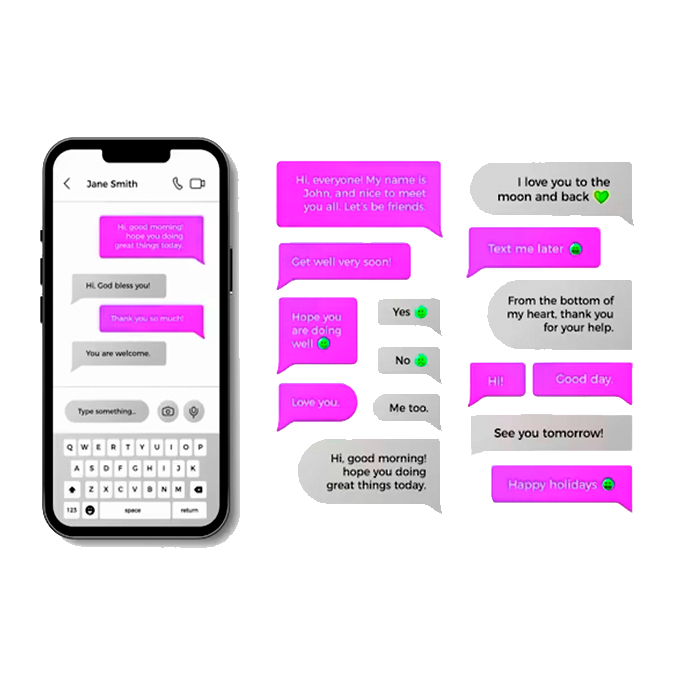
\includegraphics[width=0.7\linewidth]{images/komp_messenger}
	\caption{Композиция мессенджера}
	\label{fig:kompmessenger}
\end{figure}

\subsection{Требования пользователя к интерфейсу веб-мессенджера}

Веб-мессенджер должен обеспечивать удобное взаимодействие пользователей и предоставлять следующие возможности:
\begin{itemize}
	\item Отправка текстовых сообщений: Пользователи должны иметь возможность обмениваться текстовыми сообщениями для эффективного общения.
	\item Отправка смайликов: Возможность отправлять смайлики, обеспечивая обмен различными эмоциями.
	\item Полная авторизация для дальнейшего отображения имени в чате.
\end{itemize}

%\begin{figure}[ht]
%\caption{Композиция шаблона сайта}
%\label{templ:image}
%\end{figure}
%\vspace{-\figureaboveskip} % двойной отступ не нужен (можно использовать, если раздел заканчивается картинкой)

\subsection{Моделирование вариантов использования}
 \subsubsection{Диаграмма прецедентов}
Для разрабатываемого веб-мессенджера была реализована модель, которая обеспечивает наглядное представление вариантов использования мессенджера.

Она помогает в физической разработке и детальном анализе взаимосвязей объектов. При построении диаграммы вариантов использования применяется унифицированный язык визуального моделирования UML.

На основании анализа предметной области в программе должны быть реализованы следующие прецеденты:
\begin{enumerate}
	\item Регистрация нового пользователя.
	\item Авторизация пользователя.
	\item Отправка текстового сообщения.
	\item Прикрепление и отправка смайликов.
\end{enumerate}

\begin{figure}[ht]
	\center{\includegraphics[width=1\linewidth]{precend}}
	\caption{Диаграмма прецедентов}
	\label{precend:image}
\end{figure}

 \subsubsection{Сценарии прецедентов программы}
 
 \begin{enumerate}
 	\item Сценарий для прецедента «Регистрация нового пользователя»:
 	\begin{itemize}
 		\item основной исполнитель: пользователь;
 		\item заинтересованные лица и их требования: пользователю необходимо предоставить уникальный логин и пароль;
 		\item предусловие: пользователь открыл веб-мессенджер в браузере;
 		\item основной успешный сценарий: пользователь вводит уникальный логин и пароль, система регистрирует нового пользователя.
 	\end{itemize}
	\item Сценарий для прецедента «Авторизация пользователя»:
	\begin{itemize}
		\item основной исполнитель: пользователь;
		\item заинтересованные лица и их требования: пользователю необходимо предоставить зарегистрированный логин и пароль;
		\item предусловие: пользователь открыл веб-мессенджер в браузере;
		\item основной успешный сценарий: пользователь вводит зарегистрированный логин и пароль, система производит авторизацию.
	\end{itemize}
	
	\item Сценарий для прецедента «Отправка текстового сообщения»:
	\begin{itemize}
		\item основной исполнитель: пользователь;
		\item заинтересованные лица и их требования: пользователю необходимо написать текст сообщения;
		\item предусловие: пользователь авторизован в системе;
		\item основной успешный сценарий: пользователь вводит текст сообщения, отправляет его.
	\end{itemize}
	
	\item Сценарий для прецедента «Прикрепление и отправка смайликов»:
	\begin{itemize}
		\item основной исполнитель: пользователь;
		\item заинтересованные лица и их требования: пользователю необходимо выбрать смайлик и отправить его;
		\item предусловие: пользователь авторизован в системе;
		\item основной успешный сценарий: пользователь выбирает смайлик, отправляет его.
	\end{itemize}
	
\end{enumerate}

\subsection{Требования к оформлению документации}

Разработка программной документации и программного изделия должна производиться согласно ГОСТ 19.102-77 и ГОСТ 34.601-90. Единая система программной документации.

\section{Технический проект}
\subsection{Общая характеристика организации решения задачи}
Необходимо спроектировать и разработать веб-мессенджер в ретро-стиле для обмена текстовыми сообщениями между пользователями. Все пользователи общаются в общем групповом чате, и нет личных контактов. Серверная часть реализована на языке программирования Python с использованием SQLite 3 для хранения сообщений и информации о пользователях. Веб-клиент реализован с использованием HTML, CSS и JavaScript.

\subsection{Описание используемых библеотек и языков программирования}
Проект реализован с использованием следующих языков программирования и технологий:

\subsubsection{Серверная часть: Python}
Python используется для реализации серверной части мессенджера. Он обеспечивает взаимодействие с базой данных SQLite 3, обработку запросов от клиентов, отправку и прием сообщений.

\subsubsection{Веб-клиент: HTML, CSS, JavaScript}
Для создания веб-клиента используются технологии веб-разработки. HTML используется для структуры веб-страницы, CSS - для стилей и внешнего вида, JavaScript - для взаимодействия с сервером, обновления данных на странице и реализации интерактивности.

\subsubsection{База данных: SQLite 3}
SQLite 3 используется для хранения сообщений и информации о пользователях. Это легковесная база данных, которая интегрируется в проект и обеспечивает эффективное хранение и извлечение данных.

\subsection{Основные функции мессенджера}
Проект реализует следующие основные функции мессенджера:

\begin{itemize}
	\item Отправка сообщений: Пользователи могут отправлять текстовые сообщения в общий групповой чат.
	\item Отображение сообщений: Веб-интерфейс отображает сообщения, отправленные всеми пользователями, с указанием отправителя.
	\item Обновление сообщений в реальном времени: Новые сообщения отображаются на веб-странице без необходимости перезагрузки.
	\item Хранение сообщений и информации о пользователях: Сервер хранит сообщения и информацию о зарегистрированных пользователях в базе данных SQLite 3.

\end{itemize}

\subsection{Технические детали проекта}
\subsubsection{Обновление сообщений в реальном времени}
Для обновления сообщений в реальном времени используется технология WebSocket. Когда пользователь отправляет новое сообщение, сервер немедленно уведомляет всех подключенных пользователей о появлении нового сообщения, и их веб-страницы обновляются динамически.

\subsubsection{Авторизация пользователей}
Для обеспечения безопасности и отделения пользователей мессенджера, каждый пользователь проходит процедуру авторизации. Пользователь вводит свое имя при запуске мессенджера, и это имя используется как его идентификатор при отправке сообщений и взаимодействии с сервером.

\subsubsection{Хранение данных}
Информация о пользователях и сообщения хранятся в базе данных SQLite 3. Каждое сообщение содержит информацию об отправителе, тексте сообщения и времени отправки. Таблица пользователей содержит уникальные имена пользователей и их идентификаторы.

\subsubsection{Интерфейс веб-клиента}
Интерфейс веб-клиента состоит из области отображения сообщений и формы для отправки новых сообщений. Сообщения отображаются в хронологическом порядке с указанием имени отправителя и времени отправки. Форма отправки нового сообщения включает поле ввода текста и кнопку для отправки.


\subsection{Структура проекта}
\subsubsection{Структура серверной части}
Структура серверной части мессенджера представлена следующим образом:

\begin{figure}[H]
	\centering
	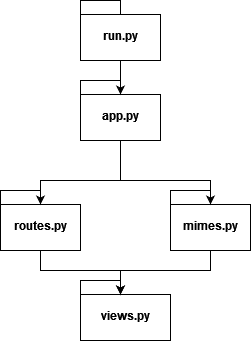
\includegraphics[width=0.7\linewidth]{images/Server_diag}
	\caption{Диаграмма компонентов сервера}
	\label{fig:serverdiag}
\end{figure}

\subsubsection{Структура веб-клиента}
Структура веб-клиента мессенджера представлена следующим образом:

\begin{figure}[H]
	\centering
	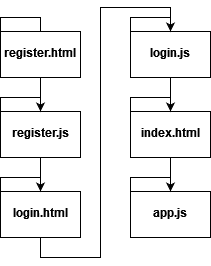
\includegraphics[width=0.7\linewidth]{images/klient_diag}
	\caption{Диаграмма компонентов веб-клиента}
	\label{fig:klientdiag}
\end{figure}

\subsubsection{Диаграмма классов}
На рисунке \ref{fig:classdiag} изображена диаграмма классов для моего проекта веб-мессенджера. Данная диаграмма визуализирует взаимодействие между различными классами, представляющими пользователей, сообщения, чаты, элементы управления и другие основные компоненты системы.


\begin{figure}
	\centering
	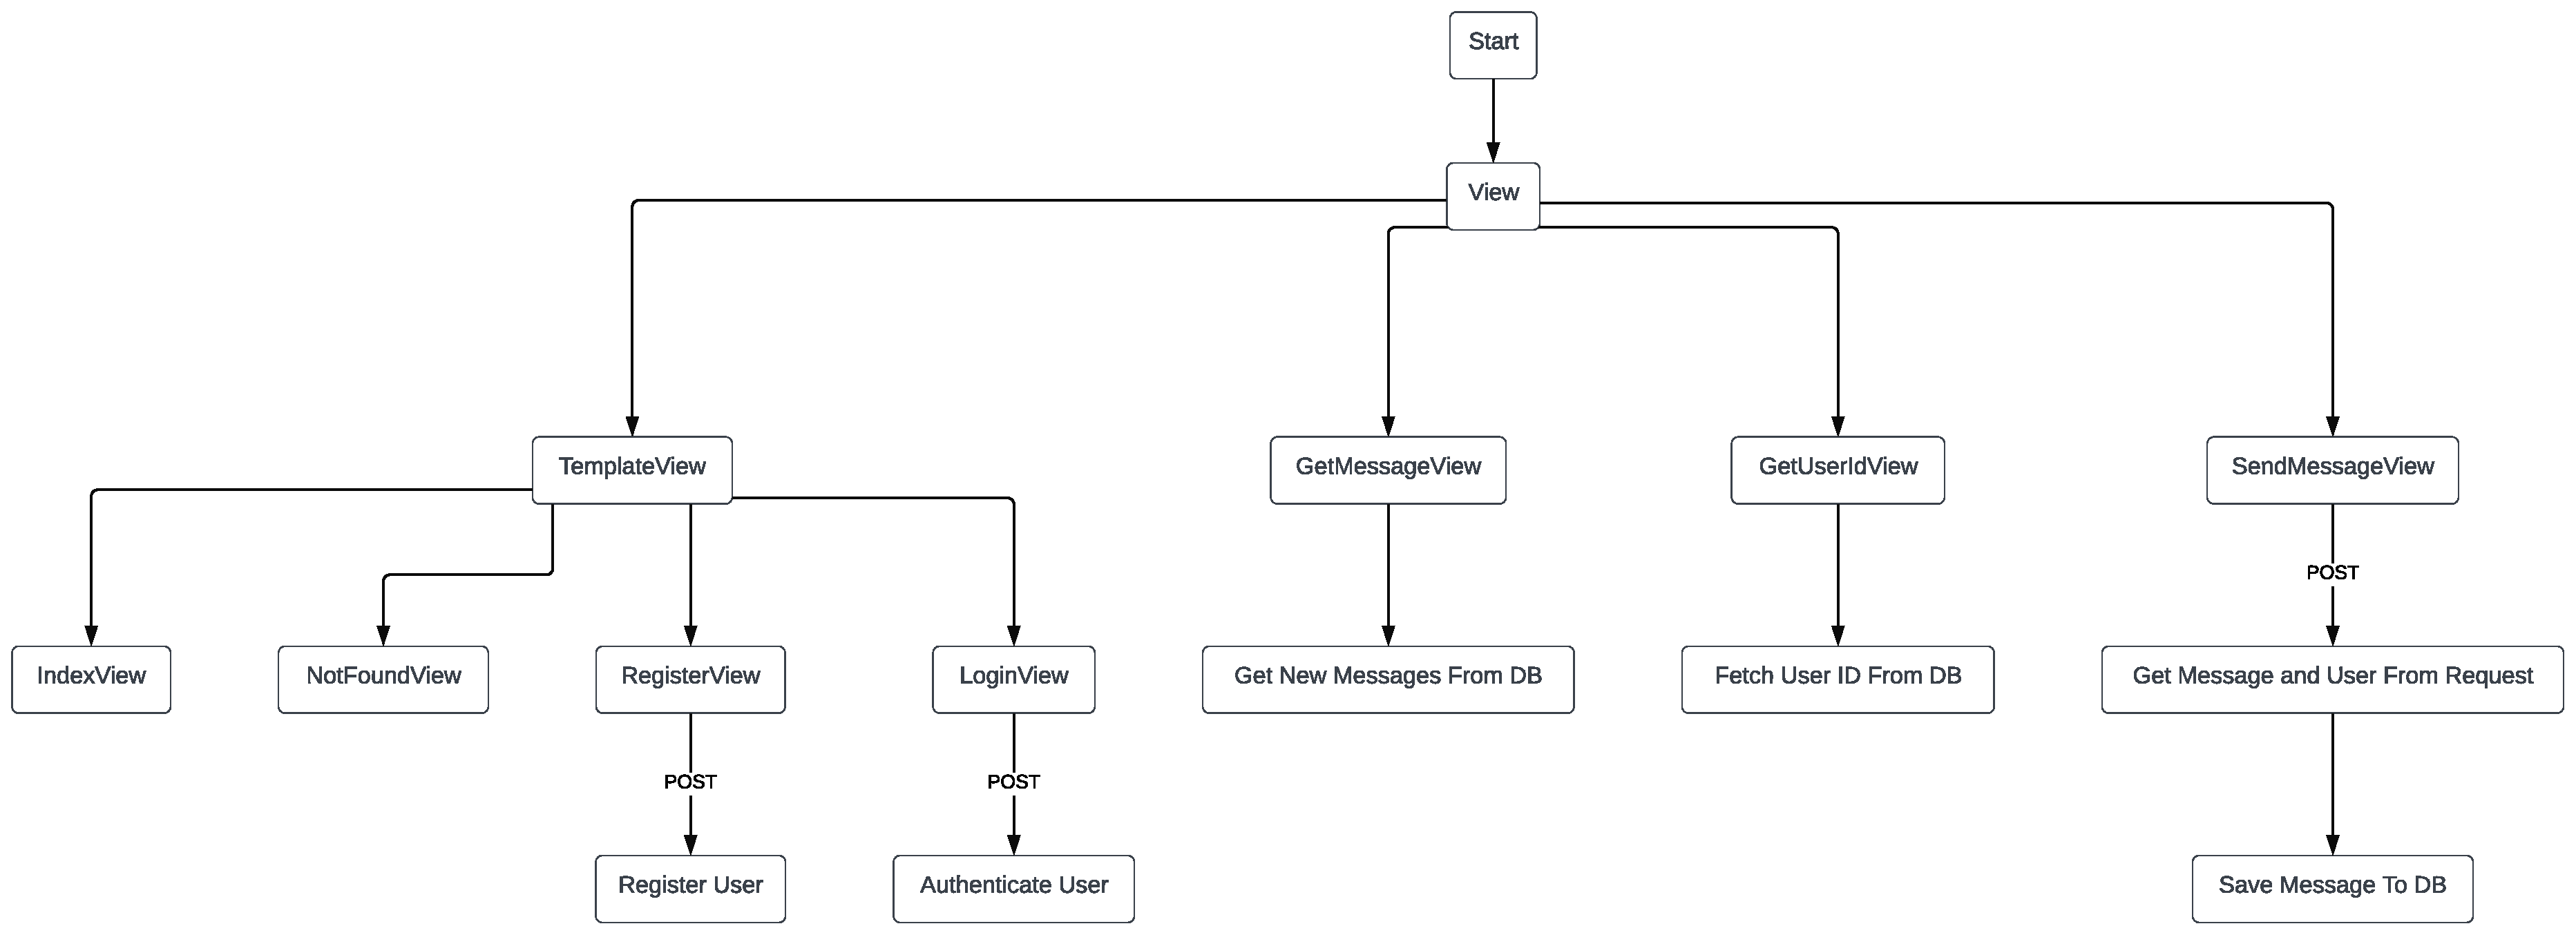
\includegraphics[width=0.7\linewidth]{images/class_diag}
	\caption{Диаграмма классов}
	\label{fig:classdiag}
\end{figure}



\ifПрактика{}\else{
   \section{Рабочий проект}
\subsection{Классы, используемые при разработке веб-мессенджера}

Можно выделить следующий список классов и их методов, использованных при разработке веб-мессенджера (таблица \ref{class:table}). Пример таблицы с уменьшенным межстрочным интервалом.

\renewcommand{\arraystretch}{0.8} % уменьшение расстояний до сетки таблицы
\begin{xltabular}{\textwidth}{|X|p{2.5cm}|>{\setlength{\baselineskip}{0.7\baselineskip}}p{4.85cm}|>{\setlength{\baselineskip}{0.7\baselineskip}}p{4.85cm}|}
	\caption{Описание классов, используемых в игре Montezuma\label{class:table}}\\
	\hline \centrow \setlength{\baselineskip}{0.7\baselineskip} Название класса & \centrow \setlength{\baselineskip}{0.7\baselineskip} Модуль, к которому относится класс & \centrow Описание класса & \centrow Методы и состояния\\
	\hline \centrow 1 & \centrow 2 & \centrow 3 & \centrow 4\\ \hline
	\endfirsthead
	\caption*{Продолжение таблицы \ref{class:table}}\\
	\hline \centrow 1 & \centrow 2 & \centrow 3 & \centrow 4\\ \hline
	\finishhead
	
	\hline \centrow App & \centrow app.py & \centrow Главный класс приложения. Отвечает за обработку HTTP-запросов и вызов соответствующих представлений. & \centrow app, load, run\\
	\hline \centrow View & \centrow views.py & \centrow Базовый класс представления. Отвечает за формирование HTTP-ответа на основе URL и запроса. & \centrow response, read\_file\\
	\hline \centrow TemplateView & \centrow views.py & \centrow Класс представления с использованием шаблона. Расширяет базовый класс View для работы с HTML-шаблонами. & \centrow response, read\_file\\
	\hline \centrow IndexView & \centrow views.py & \centrow Класс представления для главной страницы. Использует HTML-шаблон. & \centrow response, read\_file\\
	\hline \centrow NotFoundView & \centrow views.py & \centrow Класс представления для страницы 404 Not Found. Использует HTML-шаблон. & \centrow response, read\_file\\
	\hline \centrow GetMessageView & \centrow views.py & \centrow Класс представления для получения новых сообщений. Обрабатывает запросы и возвращает JSON с новыми сообщениями. & \centrow response, get\_new\_messages\_from\_db\\
	\hline \centrow GetUserIdView & \centrow views.py & \centrow Класс представления для получения идентификатора пользователя. Обрабатывает запросы и возвращает JSON с идентификатором. & \centrow response, fetch\_user\_id\_from\_database\\
	\hline \centrow SendMessageView & \centrow views.py & \centrow Класс представления для отправки сообщений. Обрабатывает запросы и сохраняет новые сообщения в базу данных. & \centrow response, save\_message\_to\_db, get\_message\_and\_user\_from\_request\\
	\hline \centrow RegisterView & \centrow views.py & \centrow Класс представления для регистрации новых пользователей. Обрабатывает запросы и регистрирует новых пользователей в базе данных. & \centrow response, register\_user, get\_post\_data\\
	\hline \centrow LoginView & \centrow views.py & \centrow Класс представления для аутентификации пользователей. Обрабатывает запросы и возвращает JSON с результатом аутентификации. & \centrow response, authenticate\_user, get\_post\_data\\
	\hline
\end{xltabular}
\renewcommand{\arraystretch}{1.0} % восстановление сетки


\subsection{Системное тестирование веб-мессенджера}

Для отладки работы веб-мессенджера разработаны следующие тестовые сценарии:

\begin{enumerate}
		\item Случай использования: регистрация нового пользователя
	\begin{itemize}
		\item Предусловие: веб-мессенджер доступен по адресу.
		\item Тестовый случай: пользователь запускает веб-мессенджер, переходя по URL с припиской /register.
		\item Ожидаемый результат: открывается страница регистрации с полем ввода логина и пароля (после успешной регистрации пользователя перекидывает на страницу /login).
		\item Результат представлен на рисунках \ref{fig:clearreg} и \ref{fig:fullreg} \ref{fig:dbadmin}.
	\end{itemize}
	
	\begin{figure}[H]
		\centering
		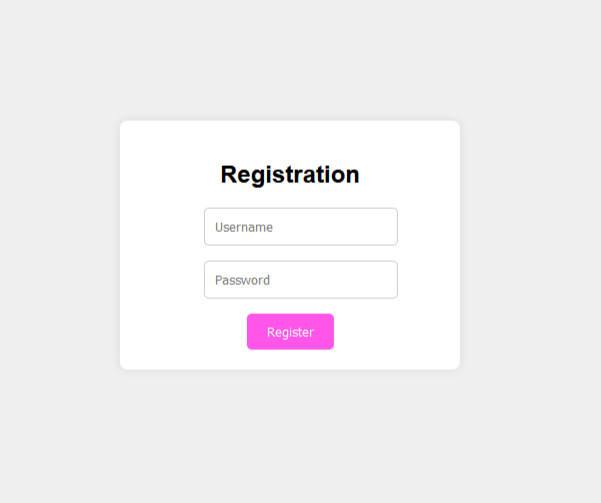
\includegraphics[width=0.7\linewidth]{images/clear_reg}
		\caption{Страница регистрации (поля пустые)}
		\label{fig:clearreg}
	\end{figure}
		
	\begin{figure}[H]
		\centering
		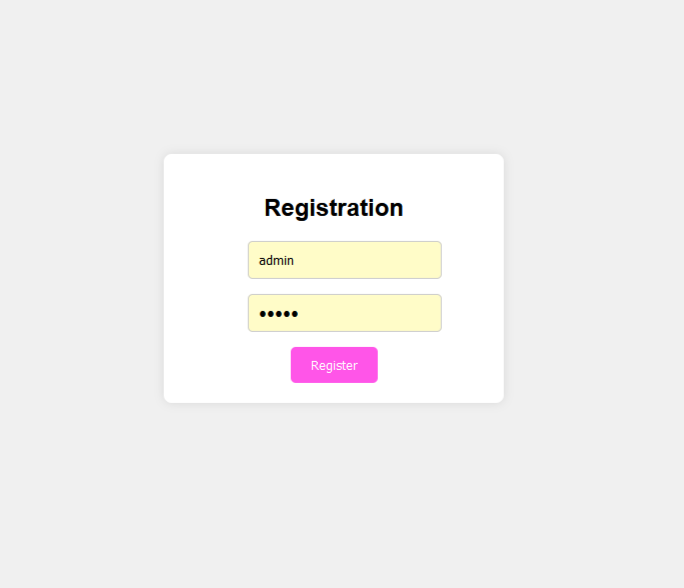
\includegraphics[width=0.7\linewidth]{images/full_reg}
		\caption{Страница регистрации (заполненные поля admin admin)}
		\label{fig:fullreg}
	\end{figure}
	
	\begin{figure}[H]
		\centering
		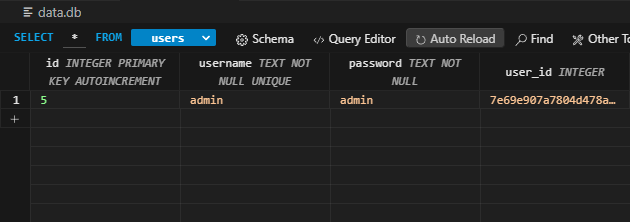
\includegraphics[width=0.7\linewidth]{images/db_admin}
		\caption{База данных после регистрации}
		\label{fig:dbadmin}
	\end{figure}
	
	\item Случай использования: логин пользователя
	\begin{itemize}
		\item Предусловие: пользователь не авторизован в системе, веб-мессенджер доступен по адресу.
		\item Тестовый случай: пользователь переходит по URL ссылке с припиской /login.
		\item Ожидаемый результат: открывается страница логина с полями для ввода логина и пароля (после успешного логина пользователя перекидывает на страницу с мессенджером).
		\item Результаты представлены на рисунках \ref{fig:clearlog} и \ref{fig:fulllog}.
	\end{itemize}
	
	\begin{figure}
		\centering
		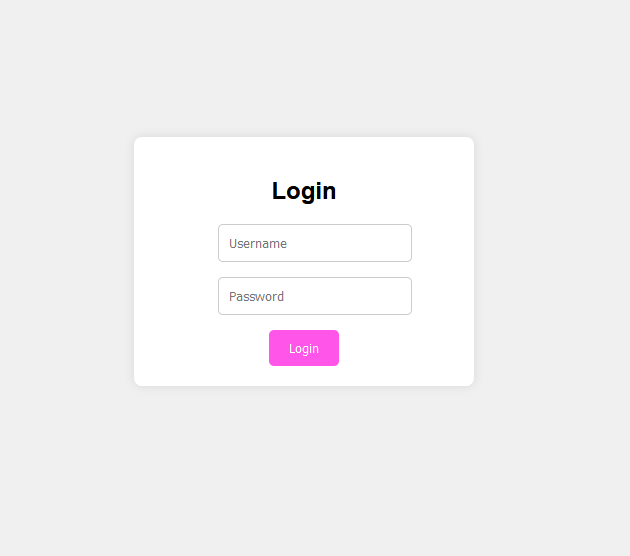
\includegraphics[width=0.7\linewidth]{images/clear_log}
		\caption{Страница логина (поля пустые)}
		\label{fig:clearlog}
	\end{figure}
	
	\begin{figure}
		\centering
		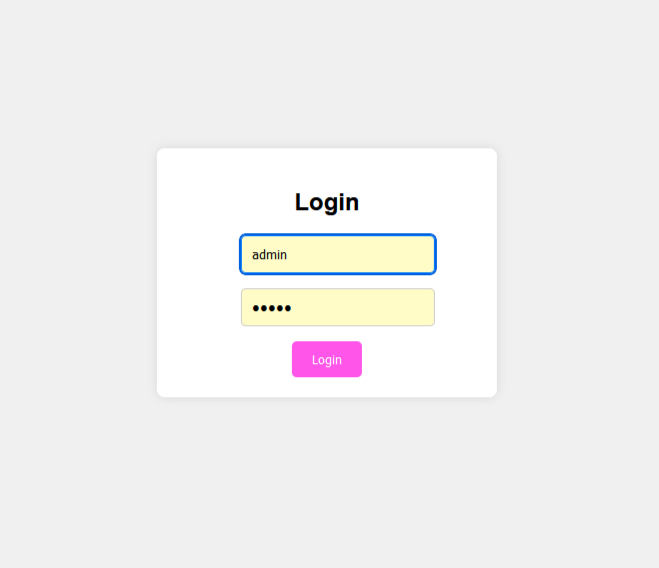
\includegraphics[width=0.7\linewidth]{images/full_log}
		\caption{Страница логина(заполненные поля admin admin)}
		\label{fig:fulllog}
	\end{figure}
		
		
	\item Случай использования: отправка сообщения (без логина)
	\begin{itemize}
		\item Предусловие: пользователь не авторизован в системе.
		\item Тестовый случай: пользователь вводит текст сообщения и нажимает кнопку "Отправить".
		\item Ожидаемый результат: сообщение отправляется, отображаемое имя Guest.
		\item Результаты представлены на рисунках \ref{fig:nonlogguestmes} и \ref{fig:dbuserclear}.
	\end{itemize}
	
	\begin{figure}[H]
		\centering
		
\includegraphics[width=0.7\linewidth]{images/nonlog_guest_mes}
		\caption{Пользователь не вошел и отправил сообщение}
		\label{fig:nonlogguestmes}
	\end{figure}
	
	\begin{figure}[H]
		\centering
		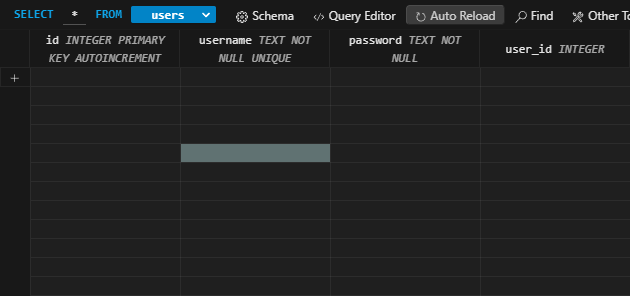
\includegraphics[width=0.7\linewidth]{images/dbuser_clear}
		\caption{Пустая база данных (зарегистрированные пользователи отсутсвуют)}
		\label{fig:dbuserclear}
	\end{figure}
	
		\item Случай использования: отправка сообщения (логин cubemalevich)
	\begin{itemize}
		\item Предусловие: пользователь авторизован в системе.
		\item Тестовый случай: пользователь вводит текст сообщения и нажимает кнопку "Отправить".
		\item Ожидаемый результат: сообщение отправляется, отображаемое имя cubemalevich.
		\item Результаты представлены на рисунках \ref{fig:logcubmes} и \ref{fig:dbmessages}.
	\end{itemize}
	
	\begin{figure}[H]
		\centering
		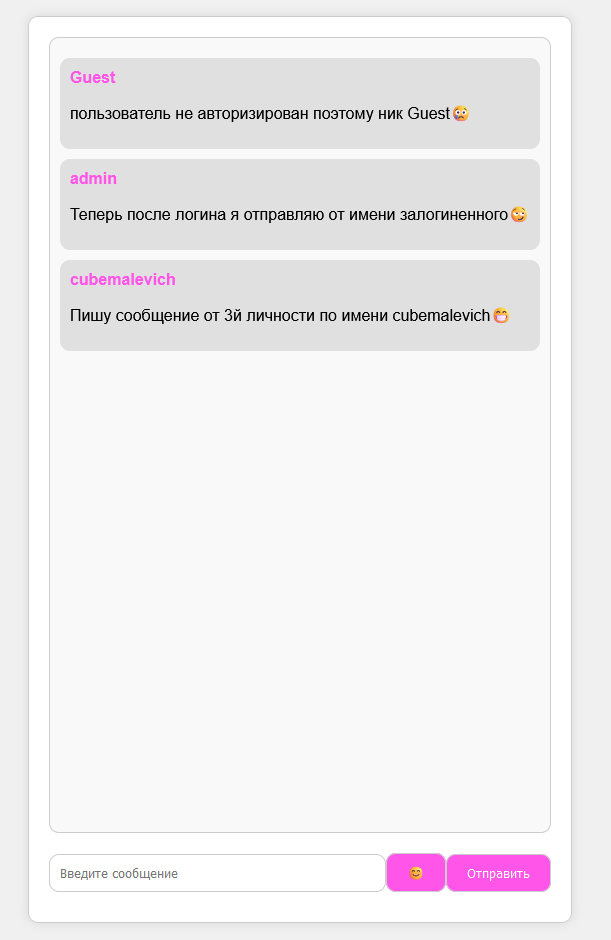
\includegraphics[width=0.7\linewidth]{images/log_cub_mes}
		\caption{Пользователь cubemalevich отправил сообщение}
		\label{fig:logcubmes}
	\end{figure}

	\begin{figure}[H]
		\centering
		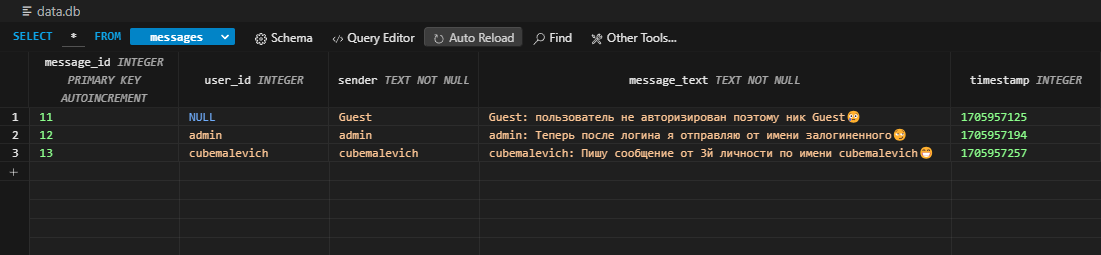
\includegraphics[width=0.7\linewidth]{images/db_messages}
		\caption{База данных с сообщениями}
		\label{fig:dbmessages}
	\end{figure}
	
	\item Случай использования: отправка смайликов
	\begin{itemize}
		\item Предусловие: пользователь авторизован в системе.
		\item Тестовый случай: пользователь нажимает кнопку отправки смайликов.
		\item Ожидаемый результат: открывается "пикер" смайликов, пользователь выбирает смайлик и отправляет.
		\item Результаты представлены на рисунках \ref{fig:smilepicker}, \ref{fig:sendsmile} и \ref{fig:dbmessagessmile}.
	\end{itemize}
	
	\begin{figure}[H]
		\centering
		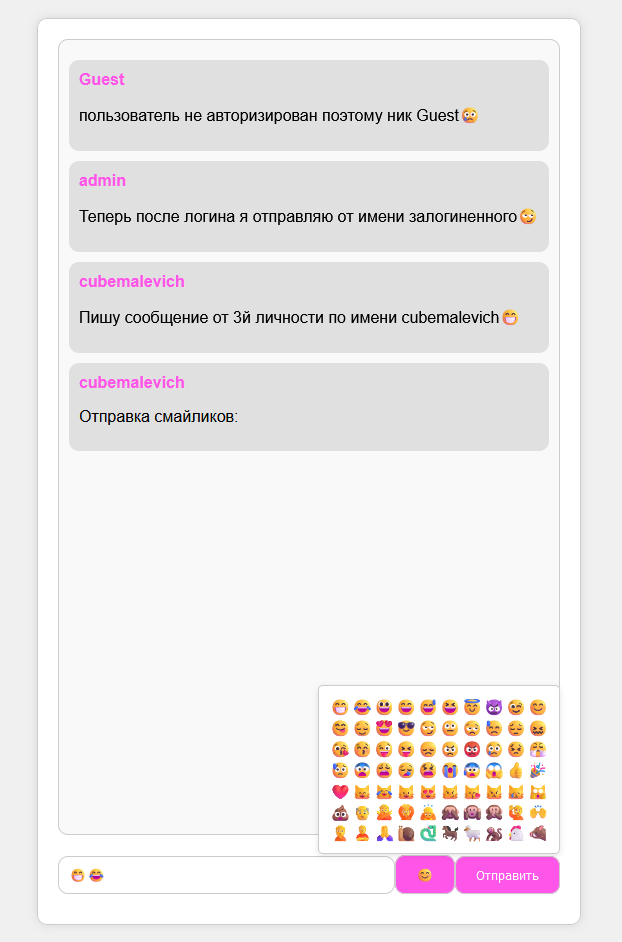
\includegraphics[width=0.7\linewidth]{images/smile_picker}
		\caption{Пикер смайликов}
		\label{fig:smilepicker}
	\end{figure}
		
	\begin{figure}[H]
		\centering
		
\includegraphics[width=0.7\linewidth]{images/send_smile}
		\caption{Отправленные смайлики}
		\label{fig:sendsmile}
	\end{figure}
	
	\begin{figure}[H]
		\centering
		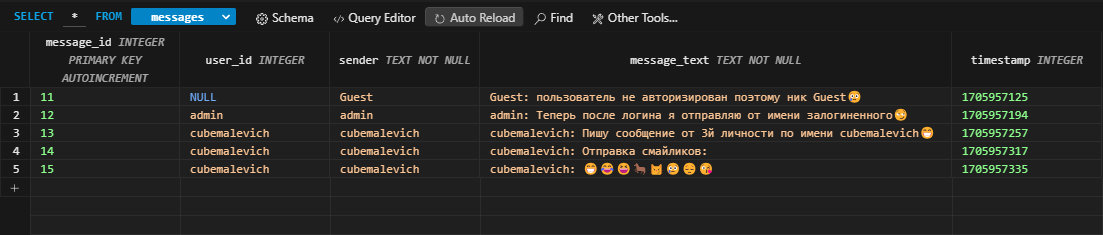
\includegraphics[width=0.7\linewidth]{images/db_messages_smile}
		\caption{База данных с сообщениями}
		\label{fig:dbmessagessmile}
	\end{figure}


\end{enumerate}

   \section*{ЗАКЛЮЧЕНИЕ}
\addcontentsline{toc}{section}{ЗАКЛЮЧЕНИЕ}

Веб-мессенджер, разработанный с использованием современных веб-технологий, представляет собой реализацию эффективного средства обмена сообщениями. Процесс разработки данного проекта позволил глубже понять принципы работы веб-приложений, взаимодействие с базой данных и создание динамического пользовательского интерфейса.

Основные результаты данного проекта включают в себя:

\begin{enumerate}
	\item Проведен анализ существующих веб-мессенджеров, выделены ключевые функциональности и принципы их реализации, которые были учтены при разработке данного проекта.
	\item Создано веб-приложение, включающее в себя возможность регистрации и авторизации пользователей, отправки и получения сообщений.
	\item Проведено тестирование веб-мессенджера, результаты которого подтвердили корректную работу основных функций приложения.
\end{enumerate}

Все изначально поставленные задачи были успешно выполнены в ходе разработки. Созданный веб-мессенджер предоставляет пользователям удобный инструмент для общения и обмена информацией.

Разработанный проект успешно реализует основные функциональности веб-мессенджера, делая его полезным и эффективным средством коммуникации.

}\fi
\addcontentsline{toc}{section}{СПИСОК ИСПОЛЬЗОВАННЫХ ИСТОЧНИКОВ}

\begin{thebibliography}{9}

    \bibitem{python} Мэтиз Э. Изучаем Python: программирование игр, визуализация данных, веб-приложения. 3-е изд. / Мэтиз Эрик 2022 ISBN 978-5-4461-1528-0. – Текст~: непосредственный.
    
    \bibitem{JavaScript} МакГрат М. JavaScript для начинающих. 6-е издание / МакГрат Майк 2023,ISBN 978-5-04-121621-4. – Текст~: непосредственный.
    
    \bibitem{python} Джейкс, Дж. Python Crash Course / Дж. Джейкс. – Санкт-Петербург : Питер, 2022. – 560 с. – ISBN 978-5-4461-2206-7.
    
    \bibitem{python} Любанович Б. Простой Python. Современный стиль программирования/ Б. Любанович – Санкт-Петербург : Питер, 2022. – 592 с. – ISBN 978-5-4461-1639-3. – Текст~: непосредственный.
    
    \bibitem{python} Бейдер Д.Знакомство с Python / Д. Бейдер. – Санкт-Петербург : Питер, 2023. – 512 с. – ISBN 978-5-4461-1924-0. – Текст~: непосредственный.
    
	\bibitem{python} Джонс Б, Бизли Д. Python. Книга рецептов /Б. Джонс, Д. Бизли – Москва~: ДМК Пресс, 2019. – 898 с. – ISBN 978-5-97060-751-0. – Текст~: непосредственный.
	
	\bibitem{python} Гринберг М. Разработка веб-приложений с использованием Flask на языке Python / Гринберг Мигель 2016. ISBN - 978-5-97060-206-5, 978-1-449-37262-0
	
	\bibitem{bigbook} Вигерс, К. Разработка требований к программному обеспечению : [практические приёмы сбора требований и управления ими при разработке программных продуктов : пер. с англ.] / К. Вигерс, Д. Битти. – 3-е изд., доп.– Санкт-Петербург, 2020. – 736 с. – ISBN: 978-5-9775-3348-5. 
	
	\bibitem{oop1} Гамма Э., Хелм Р. Паттерны объективно–ориентированного программирования/ БЭ. Гамма, Р. Хелм – Санкт-Петербург : Питер, 2021 – 448 с. – ISBN 978-5-4461-1595-2. – Текст~: непосредственный.
	
	\bibitem{oop2} Рамбо  Дж. UML 2.0. Объектно-ориентированное моделирование и разработка/ Дж. Рамбо – Санкт-Петербург : Питер, 2015 – 545 с. – ISBN 5-469-00814-2. – Текст~: непосредственный. 
	   
	\bibitem{JavaScript} Скотт Адам Д., Пауэрс Ш. JavaScript. Рецепты для разработчиков. 3-е изд / Скотт Адам Д., Пауэрс Шелли 2023.  ISBN - 978-5-4461-2001-7 – Текст~: непосредственный. 
	
	\bibitem{JavaScript} Кириченко А.;Никольский А. Web на практике. CSS, HTML, JavaScript, MySQL, PHP для fullstack-разработчиков 2023. ISBN - 978-5-94387-271-6 – Текст~: непосредственный. 
	
	\bibitem{sdl} Веб-технологии для разработчиков [Электронный ресурс] https://developer.mozilla.org/ru/docs/Web 
	
\end{thebibliography}

\ifВКР{\appendix{Представление графического материала}

Графический материал, выполненный на отдельных листах,
изображен на рисунках А.1--А.\arabic{числоПлакатов}.
\setcounter{числоПлакатов}{0}

\renewcommand{\thefigure}{А.\arabic{figure}} % шаблон номера для плакатов

\begin{landscape}

\begin{плакат}
    
\includegraphics[width=0.82\linewidth]{плакат1.png}
    \заголовок{Сведения о ВКРБ}
    \label{pl1:image}      
\end{плакат}

\begin{плакат}
    
\includegraphics[width=0.82\linewidth]{плакат2.png}
    \заголовок{Цель и задачи разработки}
    \label{pl2:image}      
\end{плакат}

\begin{плакат}
    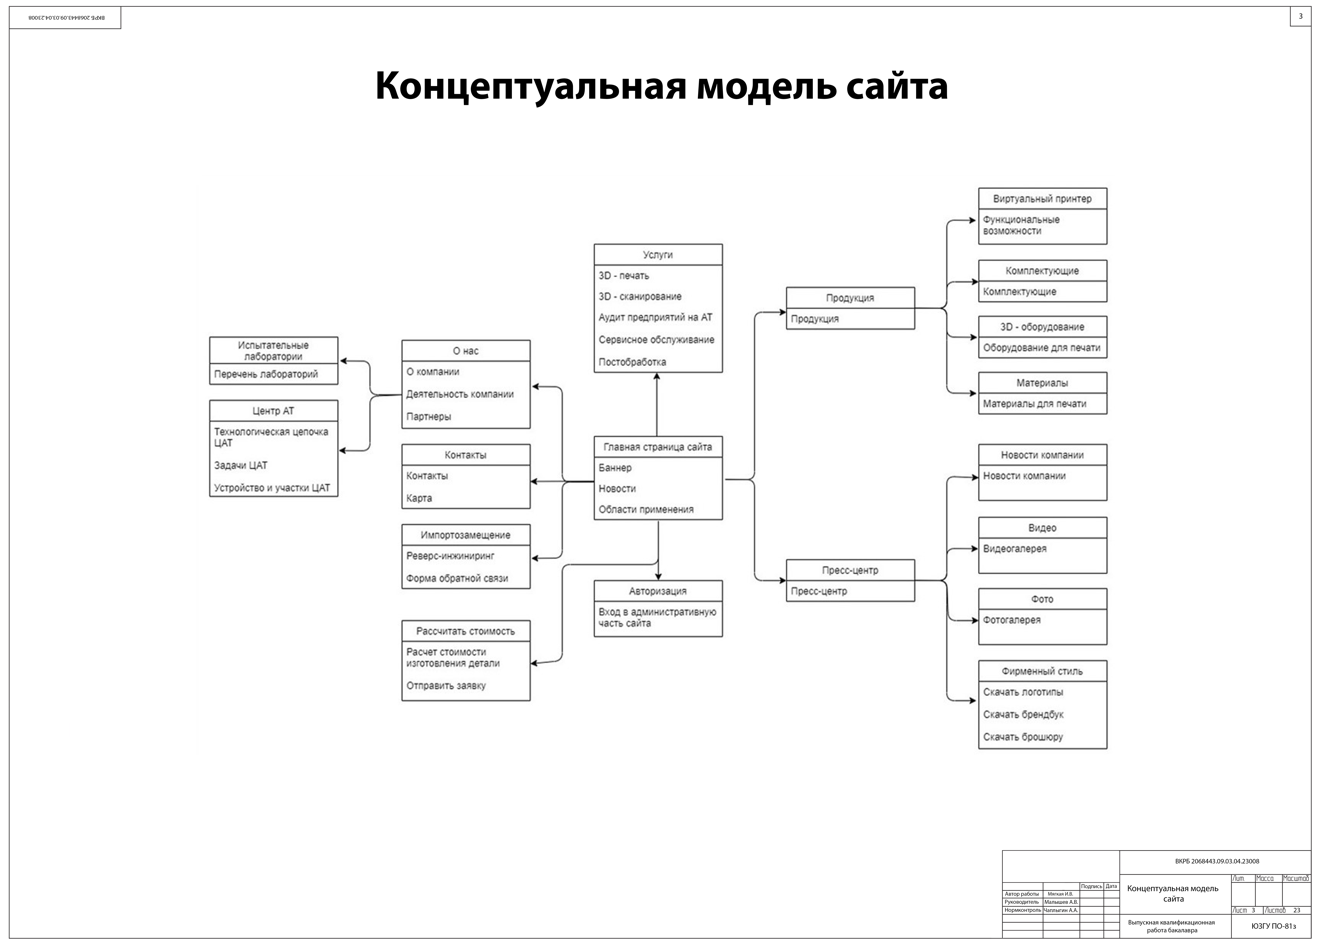
\includegraphics[width=0.82\linewidth]{плакат3.png}
    \заголовок{Концептуальная модель сайта}
    \label{pl3:image}      
\end{плакат}

\begin{плакат}
    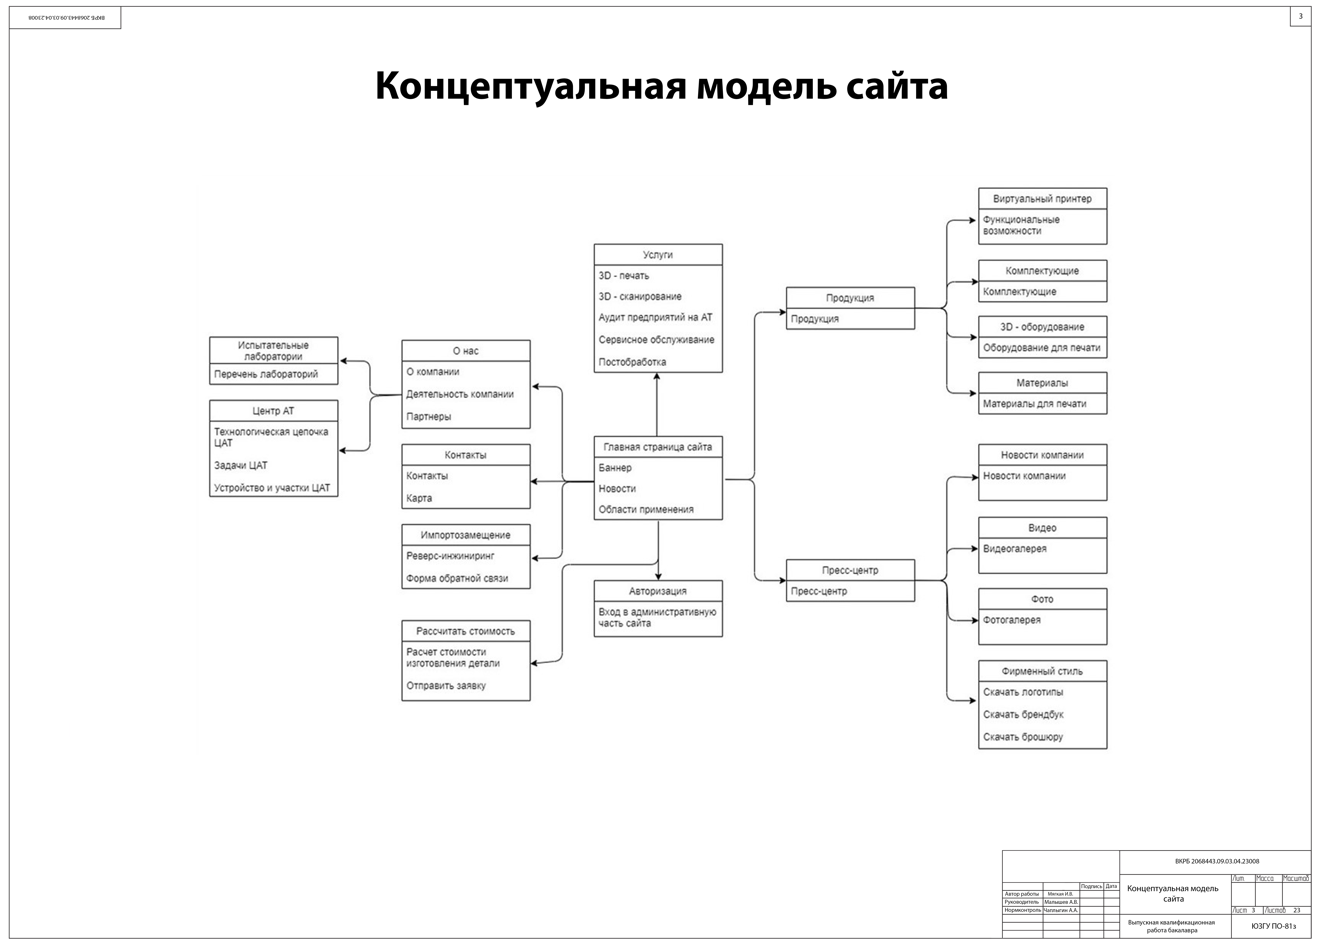
\includegraphics[width=0.82\linewidth]{плакат3.png}
    \заголовок{Еще плакат}
    \label{pl4:image}      
\end{плакат}

\end{landscape}
}\fi
\ifПрактика{}\else{\appendix{Фрагменты исходного кода программы}

app.js
\lstinputlisting[language=JavaScript, frame=none]{app.js}

login.js
\lstinputlisting[language=JavaScript, frame=none]{login.js}

register.js
\lstinputlisting[language=JavaScript, frame=none]{register.js}

index.html
\lstinputlisting[language=HTML, frame=none]{index.html}

login.html
\lstinputlisting[language=HTML, frame=none]{login.html}

register.html
\lstinputlisting[language=HTML, frame=none]{register.html}

app.py
\lstinputlisting[language=Python, frame=none]{app.py}

views.py
\lstinputlisting[language=Python, frame=none]{views.py}

mimes.py
\lstinputlisting[language=Python, frame=none]{mimes.py}

routes.py
\lstinputlisting[language=Python, frame=none]{routes.py}

run.py
\lstinputlisting[language=Python, frame=none]{run.py}


\ifВКР{
	\newpage
	\addcontentsline{toc}{section}{На отдельных листах (CD-RW в прикрепленном конверте)}
	\begin{center}
		\textbf{Место для диска}
	\end{center}
}\fi

}\fi
\end{document}
